% Document structure and styling
\documentclass[11pt]{article}

\usepackage{graphicx} % Required for including images
\usepackage{multicol} % Required for image alignment

\setlength{\parindent}{0pt} % Stop paragraph indentation
\setlength{\parskip}{1pt} % Stop paragraph indentation

%----------------------------------------------------------------------------------------
%	FONTS
%----------------------------------------------------------------------------------------

\usepackage[utf8]{inputenc} % Required for inputting international characters
\usepackage[T1]{fontenc} % Output font encoding for international characters
\usepackage[semibold]{ebgaramond} % Use the EB Garamond font with a reduced bold weight

%----------------------------------------------------------------------------------------
%	MARGINS
%----------------------------------------------------------------------------------------

\usepackage{geometry} % Required for adjusting page dimensions and margins
\geometry{
	paper=a4paper, % Paper size, change to letterpaper for US letter size
	top=2.5cm, % Top margin
	bottom=2.5cm, % Bottom margin
	left=5cm, % Left margin
	right=3cm, % Right margin
}

%----------------------------------------------------------------------------------------
%	MARGIN CONTENTS
%----------------------------------------------------------------------------------------

\usepackage{marginnote} % Required to output text in the margin
\setlength{\marginparwidth}{5cm}

%\renewcommand*{\raggedleftmarginnote}{} % Left-align the years in the margin
%\setlength{\marginparsep}{-1pt} % Move the margin content closer to the text
\reversemarginpar % Margin text to be output into the left margin instead of the default right margin

%----------------------------------------------------------------------------------------
%   NEWCOMMANDS
%----------------------------------------------------------------------------------------

% New command for adding time to the margin
\newcommand{\when}[1]{\marginnote{\small{#1}}}

% New command for adding a new entry
\newcommand{\new}[4]{
    \medbreak
    \vspace{3mm}
    \marginnote{\small #1}
    \nopagebreak
    \textbf{#2}\\
    \nopagebreak
    \textit{#3}, #4
    \medskip
    }

% New command for section heading
\newcommand{\cat}[1]{
    \bigbreak
    \vspace{5mm}
    \pagebreak[1]
    {\Large\bfseries #1}
    \nopagebreak
    }

% New command for skill entry
\newcommand{\sky}[2]{
    \vspace{1mm}
    \marginnote{\small\bfseries #1}
    #2
    }
%----------------------------------------------------------------------------------------
%	COLORED LINKS
%----------------------------------------------------------------------------------------

\usepackage[usenames, dvipsnames]{xcolor} % Required for specifying colours by name
\usepackage[colorlinks]{hyperref} % Required for links

% Set link colours
\hypersetup{
	linkcolor=blue,
	urlcolor=MidnightBlue
}


\begin{document}
\begin{multicols}{2}

{\LARGE\bfseries Albert Shaji}
\bigskip\bigskip % Whitespace

Ernakulam-686671\\
Kerala, India
\medskip

+91 8281129015\\
\href{mailto:alby@disroot.org}{alby@diroot.org}\\
\href{https://albertshaji.github.io/}{https://albertshaji.github.io}\\
\medskip

\fbox{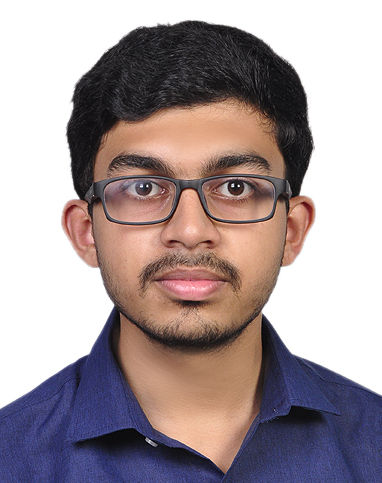
\includegraphics[width=3cm]{protrait.jpg}}

\end{multicols}

% Set PDF meta-information
\hypersetup{
	pdftitle={Albert Shaji - Curriculum vitae},
	pdfauthor={Albert Shaji}
}


\cat{Education}

\new{2016 -- 2019}
{B.Sc Physics Chemistry Mathematics}
{Christ University}
{Bangalore}

CGPA: 3.14/4.00
\medskip

\textbf{Discipline-Specific Electives}\\
Physics: Analog and Digital Electronics, Quantum Mechanics\\
Mathematics: Calculus of several variables, Graph Theory
\medskip

\textbf{Generic Electives}\\
Teaching Learning\\
Astronomy and Astrophysics\\
Health and Psycho-Physiology

\new{2014 -- 2016}
{High School - Science}
{Kendriya Vidyalaya Vikaspuri}
{New Delhi}

Percentage: 70\%
\cat{Research Experience}

\new{Aug 2019 -- Oct 2019}
{Maximum Entropy Probability Distribution}
{Raman Research Institute}
{Bangalore}

Guide: Prof. Avinash Deshpande

\new{Apr 2018 -- May 2018}
{Elliptic Functions}
{Kerala School of Mathematics}
{Kozhikode}

Guide: Prof. M Manickam

\new{Apr 2017 -- May 2017}
{Real Analysis and Metric Space}
{TIFR - Centre for Applicable Mathematics}
{Bangalore}

Guide: Prof. KT Joseph
\cat{Work Experience}

\new{Feb 2020 -- Mar 2020}
{Curriculum Developer}
{Sciensation Society}
{Hyderabad}

\medbreak
\textbf{Responsibilities}\\
Develop English and Mathematics Curriculum for middle school students.\\
Attend Brainstorming sessions on Research, Design Thinking, and Philosophy.
\cat{Honors and Awards}

\new{Mar 2014}
{Junior Mathematical Olympiad}
{Kendriya Vidyalaya Sangathan}
{New Delhi}

All India Rank: 29

\new{Sep 2014, 2013}
{Painting Competition}
{Kerala House}
{New Delhi}

Position: First
\cat{Workshops and Seminars}

\new{Oct 2019}
{Manim (Python library for Mathematics Animation)}
{Indian Institute of Science}
{Bangalore}

\new{May 2018}
{Number Theory and Algebra}
{Kerala School of Mathematics}
{Kozhikode}

\new{Mar 2018}
{Python Programming}
{Christ University}
{Bangalore}

\new{Feb 2018}
{Mathematical Analysis}
{Christ University}
{Bangalore}

\new{Nov 2017}
{Amateur Radio}
{Indian Institute of Hams}
{Bangalore}

\new{Feb 2017}
{Stellar Astrophysics}
{Christ University}
{Bangalore}
\cat{Skills}
\bigskip

\sky{Languages}
{English (Fluent), Malayalam (Native), Hindi (Fluent)}

\sky{Software}
{Linux, SciLab, Maxima}

\sky{Programming}
{Python (Intermediate), C++ (Advanced)}

\sky{Markup}
{LaTeX (Advanced), HTML-CSS (Intermediate)}

% Set PDF meta-information
\hypersetup{
	pdftitle={Albert Shaji - Curriculum vitae},
	pdfauthor={Albert Shaji}
}
\end{document}
